
\documentclass[a4paper,11pt]{article}

\usepackage[utf8x]{inputenc}
\SetUnicodeOption{mathletters}
\SetUnicodeOption{autogenerated}


\usepackage{lmodern}
\renewcommand*\familydefault{\sfdefault} %% Only if the base font of the document is to be sans serif
\usepackage[T1]{fontenc}


\usepackage[italian]{babel}
\usepackage{booktabs}
\usepackage{mathpazo}
\usepackage{graphicx}
\usepackage[left=2cm, right=2cm, bottom=3cm]{geometry}
\frenchspacing

\begin{document}
\noindent {\Large ABC 2014}
\vspace{0.5cm}

\noindent{\Huge Semina del campo (\texttt{semina})}


\section*{Descrizione del problema}

Il giardiniere Mario è nel periodo dell'anno dove lavora di più: la primavera. \\
Il suo compito è seminare l'erba di un nuovo campo da calcio. \\
Essendo molto pigro, Mario non riesce a completare la semina del campo in un'unica volta e deve quindi tornarci. Sfortunatamente per lui è anche molto distratto e non riesce a ricordarsi esattamente quali parti del campo ha già seminato e può quindi capitare che in una delle volte successive rimetta i semi in parti dove aveva già seminato.\\
Aiuta Mario a capire quanti semi ha messo, al termine di tutte le semine, nella zona dove ve ne sono di più.\\\\
Il campo da seminare è suddiviso in quadrati di lato \textbf{1} metro utilizzando un sistema di coordinate cartesiane con origine nel centrocampo. \textbf{Un'unità del piano cartesiano corrisponde a 1 metro di campo}.\\
Ogni volta che Mario semina copre una zona rettangolare mettendo esattamente \textbf{1} seme in ognuno dei quadrati che compongono la zona.
\section*{Dati di input}
L'input è costituito da 1 + N linee.\\
La prima linea è costituita da un unico numero intero positivo \textbf{N}, il numero di semine che Mario ha effettuato sul campo.\\
Le successive N linee sono costituite da 4 interi ($Xi$, $Yi$, $Xf$, $Yf$): le coordinate del vertice in alto a sinistra e del vertice in basso a destra della i-esima zona rettangolare di campo seminata.

\section*{Dati di output}
  
L'output è costituito da un unico numero intero non negativo: quanti semi Mario ha messo, al termine di tutte le semine, nella zona dove ve ne sono di più.

  \section*{Assunzioni}
  \begin{itemize}
  \item $1 \leq N \leq 100$.
  \item $-100 < Xi, Yi, Xf, Yf < 100$.
\item Per ogni semina, vale che $Xi < Xf$ e $Yf < Yi$.

  \end{itemize}

\section*{Esempi di input/output}

  
    \noindent
    \begin{tabular}{p{8cm}|p{8cm}}
    \toprule
    \textbf{Input \texttt{(stdin)}}
    & \textbf{Output \texttt{(stdout)}}
    \\
    \midrule
    \small
    \begin{verbatim}
2
2 5 6 2
0 5 3 1
      \end{verbatim}
    &
    \small
    \begin{verbatim}
2
\end{verbatim}
    \\
    \bottomrule
    \end{tabular} \\[12pt]
Nel caso di esempio mostrato, l'area tra (2, 5) e (3, 2) è stata seminata due volte.\\
L'immagine sotto riportata esemplifica il caso di input.\\[1cm]
\centerline{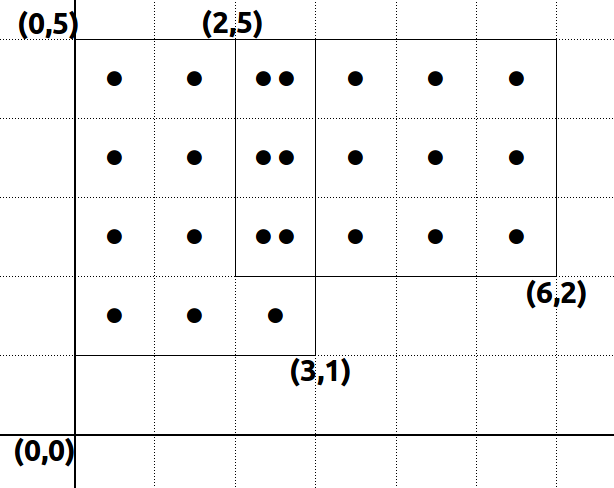
\includegraphics[width=10cm]{image.png}}



\end{document}
